\begin{figure}
\centering
\scalebox{.8}{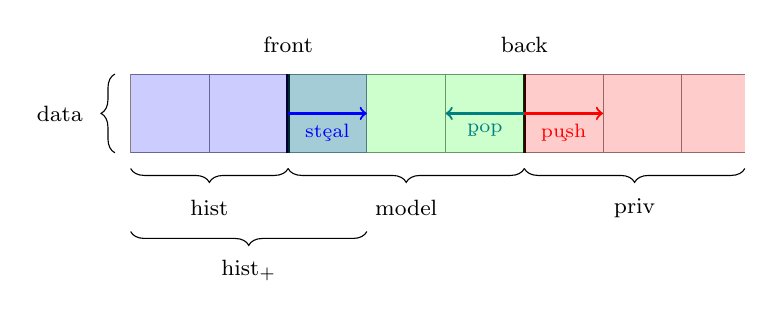
\begin{tikzpicture}
  \def\hist{2}
  \def\histx{1}
  \def\model{3}
  \def\priv{2.8}

  \draw[step=1cm, gray] (0, 0) grid ++(\hist + \model + \priv, 1) ;
  \draw[decorate, decoration={brace, amplitude=5pt}] (-0.2, 0) -- ++(0, 1) node [midway, xshift=-7mm] {\footnotesize data} ;

  \draw[very thick] (\hist, 0) -- ++(0, 1) node[label=above:\footnotesize front] {} ;

  \draw[very thick] (\hist + \model, 0) -- ++(0, 1) node[label=above:\footnotesize back] {} ;

  \fill[red, opacity=0.2] (\hist + \model, 0) rectangle ++(\priv, 1) ;
  \draw[decorate, decoration={brace, amplitude=5pt}] (\hist + \model + \priv, -0.2) -- ++(- \priv, 0) node [midway, yshift=-5mm] {\footnotesize priv} ;

  \fill[green, opacity=0.2] (\hist, 0) rectangle ++(\model, 1) ;
  \draw[decorate, decoration={brace, amplitude=5pt}] (\hist + \model, -0.2) -- ++(- \model, 0) node [midway, yshift=-5mm] {\footnotesize model} ;
  \fill[blue, opacity=0.2] (0, 0) rectangle ++(\hist, 1) ;
  \draw[decorate, decoration={brace, amplitude=5pt}] (\hist, -0.2) -- ++(- \hist, 0) node [midway, yshift=-5mm] {\footnotesize hist} ;

  \fill[blue, opacity=0.2] (\hist, 0) rectangle ++(\histx, 1) ;
  \draw[decorate, decoration={brace, amplitude=5pt}] (\hist + \histx, - 1) -- ++(- \hist - \histx, 0) node [midway, yshift=-5mm] {\footnotesize hist\textsubscript{+}} ;

  \draw[thick, ->, blue] (\hist, 0.5) -- ++(1, 0) node[midway, below] {\scriptsize\c{steal}} ;

  \draw[thick, ->, teal] (\hist + \model, 0.5) -- ++(- 1, 0) node[midway, below] {\scriptsize\c{pop}} ;
  \draw[thick, ->, red] (\hist + \model, 0.5) -- ++(1, 0) node[midway, below] {\scriptsize\c{push}} ;
\end{tikzpicture}}
\caption{\ocamlinline{Inf_ws_deque}: Physical state}
\label{fig:chaselev_inf_ws_deque_physical_state}
\end{figure}
